\documentclass[12pt]{article}

\usepackage{times}
\usepackage{graphicx}
\usepackage{amsmath}
\usepackage{url}

\setlength{\textwidth}{6.5in}
\setlength{\textheight}{8.9in}
\setlength{\oddsidemargin}{0.0in}
\setlength{\topmargin}{0.05in}
\setlength{\headheight}{-0.05in}
\setlength{\headsep}{0.0in}

\newcommand{\indep}{\perp\!\!\!\perp}

\begin{document}

\begin{center}
{\bf CS 6300} \hfill {\large\bf HW07: Bayes Nets I \hfill Due April 4, 2017}
\end{center}

\noindent
Please use the \LaTeX\ template to produce your writeups. See the
Homework Assignments page on the class website for details.  Hand in
at: \url{https://webhandin.eng.utah.edu/index.php}.

\section{D-Separation}
 
Based only on the structure of the Bayes' Net given below,
circle whether the following conditional independence assertions are
guaranteed to be true, guaranteed to be false, or cannot be determined
by the structure alone.

\begin{center}
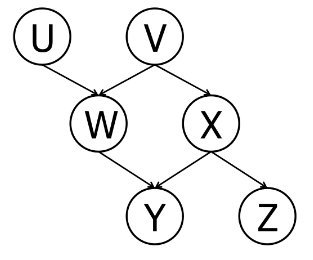
\includegraphics[height=2in]{prob1.png}
\end{center}

\begin{enumerate}

\item $U \indep V$

Guarenteed True

\item $U \indep V \mid W$

Cannot be determined

\item $U \indep V \mid Y$

Cannot be determined

\item $U \indep Z \mid W$

Cannot be determined

\item $U \indep Z \mid V, Y$

Cannot be determined

\item $U \indep Z \mid X, W$

Guarenteed True

\item $W \indep X \mid Z$

Cannot be determined

\item $V \indep Z \mid X$

Guarenteed True

\end{enumerate}

\clearpage

\section{Inference by Enumeration}

\begin{center}
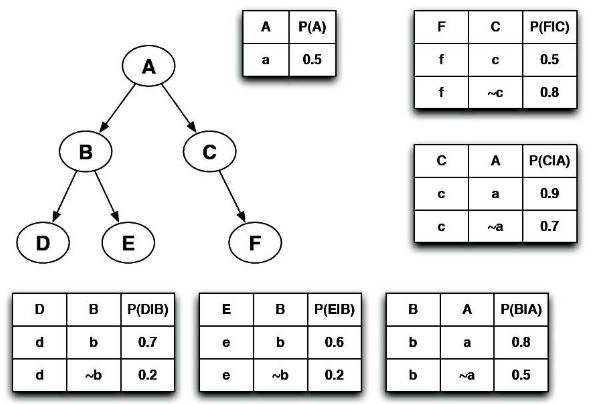
\includegraphics[width=5in]{prob2.png}
\end{center}

\begin{enumerate}

\item What is the expression for $P(A,B,C,D,E,F)$ given the structure
  of this Bayes' net and conditional probability tables?

This can be derived by just looking at the parents of each node, only encoding {\em local} interactions

\vspace{-2em}
\begin{align*}
  P(A,B,C,D,E,F) &= P(A)P(C|A)P(F|C)P(B|A)P(D|B)P(E|B)
\end{align*}

\item Perform inference by enumeration on the above network to figure
  out $P(C)$ given $F=f$ and $D= \sim d$.  Do this by using factors.
  Please give the details of your derivation.

  We can solve for $P(C)$ by summing over all the hidden variables $(a,e,b)$, giving

\begin{align*}
  P(C,f, \sim d) &= \sum_{a,b,e}P(C,f,\sim d, a, e, b)\\
                 &= \sum_{a,b,e}P(C|a)P(\sim d | b)P(f|C) P(a) P(b|a) P(e|b)\\
                 &= P(+a)P(+b|+a)P(C|+a)P(+e|+b)P(f|C)P(\sim d|+b)\\
                 &\phantom{aa}+ P(+a)P(-b|+a)P(C|+a)P(+e|-b)P(f|C)P(\sim d|-b)\\
                 &\phantom{aa}+ P(+a)P(+b|+a)P(C|+a)P(-e|+b)P(f|C)P(\sim d|+b)\\
                 &\phantom{aa}+ P(-a)P(+b|-a)P(C|-a)P(+e|+b)P(f|C)P(\sim d|+b)\\
                 &\phantom{aa}+ P(-a)P(-b|-a)P(C|-a)P(+e|-b)P(f|C)P(\sim d|-b)\\
                 &\phantom{aa}+ P(-a)P(-b|-a)P(C|-a)P(-e|-b)P(f|C)P(\sim d|-b)\\
                 &\phantom{aa}+ P(+a)P(-b|+a)P(C|+a)P(-e|-b)P(f|C)P(\sim d|-b)\\
                 &\phantom{aa}+ P(-a)P(+b|-a)P(C|-a)P(-e|+b)P(f|C)P(\sim d|+b)
\end{align*}

We also need the values for $P(\sim d|b) = 0.3$, $P(\sim d | \sim b) = 0.8$, $P(\sim e | b) = 0.4$, $P(\sim e | \sim b) = 0.8$, $P(\sim b | a) = 0.2$, $P(\sim b | \sim a) = 0.5$, $P(\sim c | a) = 0.1$, $P(\sim c | \sim a) = 0.3$, $P(\sim f | c) = 0.5$, $P(\sim f | \sim c) = 0.2$. Using these values, derived from the given tables and plugging int the equation above gives

\[
  P(c,f,\sim d) = 0.19
\]

Now, in solving for $\sim c$, where we can use the above equations again but substitute $\sim c$ in for every value of $C$ gives

\[
  P(\sim c, f, \sim d) = 0.09
\]

Finally, we have to renormalize the above equation where we take the sum of $c$ and $\sim c$ and use this as the divisor in the total. In other words...

\begin{align*}
  P(c|f, \sim d) &= \frac{\sum_{a,b,e}P(c|f,\sim d)}{\sum_{C}P(C | f, \sim d)}\\
                 &= (0.19)/(0.19 + 0.09) = 0.68\\
  P(\sim c| f, \sim d) &= \frac{\sum_{a,b,e}P(\sim c|f,\sim d)}{\sum_{C}P(C | f, \sim d)}\\
                       &= (0.09)/(0.19+0.09) = 0.32
\end{align*}

\end{enumerate}

\end{document}


